\section{Grundlagen zu \LaTeX{}}
\label{sec:grundlagen}

\subsection{Was ist \LaTeX{}?}
\label{sec:was_ist_latex}

\TeX{} ist ein Textsatzsystem von Donald E. Knuth, das 1978 veröffentlicht wurde. Es ist besonders für das Erstellen von wissenschaftlichen Dokumenten geeignet, da es viele Funktionen zur Verfügung stellt, die das Verfassen und Setzen von wissenschaftlichen Texten erleichtern. Dazu gehören beispielsweise die automatische Nummerierung von Kapiteln, Abschnitten und Abbildungen, die Erstellung von Literaturverzeichnissen und die Verwendung von mathematischen Formeln.

\LaTeX{} ist eine Sammlung von Makros für \TeX{}, die 1984 von Leslie Lamport entwickelt wurden. Es erleichtert die Verwendung von \TeX{} und bietet viele zusätzliche Funktionen, die das Erstellen von Dokumenten erleichtern.


\subsection{Verwendung von \LaTeX{}}
\label{sec:verwendung_von_latex}
Um \LaTeX{} zu verwenden, werden folgende Elemente benötigt:

Eine \textbf{\LaTeX{}-Distribution} wie TeX Live (für Linux, Windows, macOS), MiKTeX (für Windows) oder MacTeX (für macOS), Datei die notwendigen Befehle, Pakete, etc. verfügbar macht.

Einen \textbf{Texteditor} wie TeXworks, TeXstudio, Overleaf oder Visual Studio Code um \LaTeX{}-Dokumente zu erstellen und zu bearbeiten.

Im folgenden werden zwei Varianten zur Verwendung von \LaTeX{} vorgestellt:

\subsubsection{Visual Studio Code mit TeX Live}
\label{sec:visual_studio_code_mit_tex_live}
Visual Studio Code ist ein kostenloser, quelloffener Code-Editor von Microsoft, der viele Funktionen für die Entwicklung von Software bietet. Mit der Erweiterung \texttt{LaTeX Workshop} kann Visual Studio Code auch zum Erstellen von \LaTeX{}-Dokumenten verwendet werden. Die Software kann \href{https://code.visualstudio.com/Download}{hier} beim Hersteller heruntergeladen werden.

Die Erweiterung \texttt{LaTeX Workshop} kann über den \texttt{Extensions}-Tab in Visual Studio Code installiert werden.
\begin{figure}[H]
    \centering
    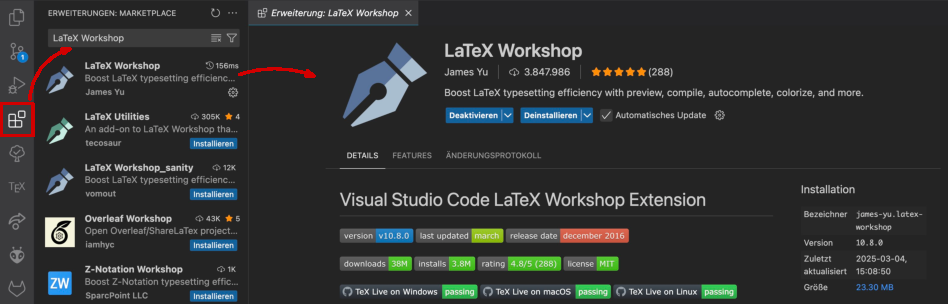
\includegraphics[width=0.8\textwidth]{anlagen/bilder/Latex_Workshop_Ext.pdf}
    \caption{Erweiterung \texttt{LaTeX Workshop}}
    \label{fig:visual_studio_code_latex_workshop}
\end{figure}

Tex Live .....
später in VSC einbinden













ggf. latexindent


\subsubsection{Overleaf}
\label{sec:overleaf}



































\newpage